\documentclass{report}

\usepackage[utf8]{inputenc}
\usepackage[francais]{babel}
\usepackage{url}
\usepackage{listings}
\usepackage{graphicx}
\title{TER, développement d'un émulateur de GameBoy}
\author{BERGER Mickaël \\ DIVET Joachim \\ VINARD Florian}
\date{17 Mai 2013}

\begin{document}
\maketitle

\tableofcontents
\chapter*{Introduction}
	Dans le cadre de la 1ère année de Master Informatique à l'Université de Montpellier
	2, tous les élèves de la promotion ont été amenés à réaliser un projet
	sous tutelle, afin de mettre en pratique les compétences acquises
	durant nos précédentes années d'études, mais aussi et surtout de nous
	placer dans un contexte de réel travail sur un projet à réaliser.\\
	Ce Travail d'Étude et de Recherche est donc un bon moyen de nous
	familiariser avec le type de travail qui pourra nous être demandé dans
	les années à venir, ainsi que de travailler nos démarches.
	Et c'est sur l'élaboration d'un Émulateur de console de jeu vidéo, et plus précisément de GameBoy,
	que nous avons choisi de travailler, plus que motivé par l'apport de
	connaissances que représente l'étude du comportement d'un processeur
	et sa simulation à partir de zéro.
	\\
	L'idée principale n'étant pas simplement de pouvoir rejouer aux jeux
	ayant bercé notre enfance, mais bien d'analyser et comprendre le
	fonctionnement d'un système d'émulation, qui reste très orienté bas
	niveau et "culture des composants", mais suffisamment accessible pour
	que notre travail puisse aboutir à un exemple concret, réalisé par nos
	soins.\\
	\\

\section*{Définition du projet}
	Dès lors que notre choix fut fixé et validé par nos enseignants, il
	fut assez rapide de déterminer les grandes lignes du déroulement du
	projet, à savoir une première étape de documentation importante, afin
	de bien comprendre le fonctionnement de l'appareil. Une seconde partie
	de développement et donc de réelle simulation des différents aspects
	du système, et une dernière partie de perfectionnement et
	amélioration éventuelle de ce que nous aurons réalisé.

\chapter{Organisation du projet}
\section{Choix des outils}
Ce projet a été réalisé grâce à de nombreux outils, les voici, avec les raisons qui ont motivés nos choix.\\

\subsection{Environnement de travail}
Linux, car il est confortable pour les développeurs. Linux dispose dans la plupart des distributions classiques d'un ensemble d'outils pour développer tel que gcc, gdb. De plus l'installation de librairies et ou de logiciels supplémentaires est relativement aisée grâce aux systèmes de logithèques.

\subsection{Langage}
C, un des langages les plus utilisés dans le monde de l'émulation. Il permet d'obtenir des exécutables compilés rapides, et selon les compilateurs de mettre en place des stratégies d'optimisations, afin de rendre l'émulateur plus fluide et rapide.

\subsection{Compilateur}
gcc, compilateur du langage C, il accepte beaucoup d'options permettant d'optimiser l'exécutable compilé.

\subsection{Librairie multimédia}
SDL, une librairie multimédia pour le langage C. Elle dispose d'un ensemble de primitives permettant de gérer tout ce qui est nécessaire pour créer un jeu en 2D et donc un émulateur de GameBoy: affichage de fenêtre, son, interruptions et autres.

\subsection{Dépôt}
Github, un site permettant de créer gratuitement un dépôt git. git est un logiciel de contrôle de version, permettant aux membres d'un même projet de modifier ce projet, en faisant en sorte que chacun puisse travailler sur la même version.

\subsection{IDE}
Le projet n'a pas été conçu avec un IDE particulier. Lors de la conception du projet il a été propre à chacun d'utiliser l'IDE qui lui convient. Cependant la plupart du code a été édité avec l'éditeur de texte vim.
\section{Documentation}
\section{Etude de l'existant}
Il existe actuellement de nombreux émulateurs de GameBoy, le but de ce projet n'était pas de rendre groboy un émulateur de renommée (d'ailleurs en quelques mois qui pourrait y'arriver?), mais bien de comprendre les rouages d'un émulateur de console de jeu.
Tous ces émulateurs ont leurs avantages par rapport aux autres. Voici une liste non exhaustive des émulateurs que nous avons trouvé intéressants, vous pourrez retrouver une liste plus complète des émulateurs GameBoy sur le site de Zophar \cite{zophar}:

\subsection{Gambatte}
Gambatte \cite{gambatte} est un émulateur open source écrit en c++, un des émulateurs les plus fidèles au comportement de la GameBoy, il se base sur des tests réalisés directement sur une GameBoy. Il émule tout aussi bien la GameBoy Color.
\subsection{Visual Boy Advance}
Visual Boy Advance \cite{visualboyadv} est un émulateur qui supporte GameBoy, GameBoy Color et GameBoy Advance. Il a été porté sur Windows, Linux et Mac.
\subsection{No\$GMB}
No\$GMB \cite{nogmb} est un émulateur de GameBoy, GameBoy Color fonctionnant sous DOS/Windows. Il est écrit en pur assembleur et est très orienté optimisation, il est donc supporté par de vieux ordinateurs avec des processeurs i386 de 33MHz.
\section{Articles de recherches}

\chapter{Etude du Hardware}
\section{CPU}
\subsection{Caractéristiques générales}
Le CPU de la GameBoy est un processeur 8 bits "Zilog 80" modifié, simplifié et adapté pour la GameBoy, son vrai nom est Sharp LR35902.
Une de ses spécificités est qu'il est capable de faire des opérations 16 bits.
Il est cadencé à 4,194304 MHz, et possède un peu moins de 512 opérations possibles.
\subsection{Registres}

Un registre interne est un espace mémoire interne au CPU, ce qui donne au CPU un accés en temps réel à cet espace mémoire. Aucun autre composant ne peut y accéder.
Le LR35902 possède 10 registres internes: 2 registres 16 bits PC et SP, et 8 registres 8 bits A, F, B, C, D, E, H, L.
Ce CPU est capable pour certaines opérations de coupler certains registres tels A et F, B et C, D et E, H et L, pour en faire des registres 16 bits, AF, BC, DE, HL.
Pratiquement tous les registres ont des rôles spécifiques:\\\\
Le registre PC appelé "Program Counter" est le registre pointant vers la prochaine instruction à effectuer.\\\\
Le registre SP appelé "Stack Pointer" est le registre pointant vers le sommet de la pile.\\\\
Le registre A appelé "Accumulator" est celui dans lequel la plupart des résultats des opérations sont stockés.\\\\
Le registre F appelé "Flags" est modifié par certaines circonstances.
Il possède 4 drapeaux, Z, N, H, C. Un drapeau n'est rien d'autre qu'un certain bit activé ou non, mais qui a une signification spécifique.
Le registre F étant rappelons le, un registre 8 bits, seuls les 4 bits de hauts niveaux servent pour les drapeaux, 
ils sont disposés tels quels: \\Z N H C - - - -.\\Les 4 bits de bas niveaux sont eux toujours à 0.
Généralement, \\Le drapeau Z est à 1 lorsque le résultat d'une opération vaut 0, 0 sinon.\\
Le drapeau N est à 1 lorsque l'opération est une soustraction, 0 pour une addition, sinon il garde son état.\\
Le drapeau H est à 1 après une opération où les 4 bits de poids faibles de l'opérande ont subi un "débordement", dépassant 0xF, le drapeau est à 0 sinon.\\
Le drapeau C est à 1 après une opération où l'opérande a subi un débordement, dépassant 0xFF, le drapeau est à 0 sinon.\\\\
Les autres registres n'ont pas vraiment de rôles spécifiques mais servent pour beaucoup d'opérations.
\subsection{Instructions}
Une instruction est un calcul ou un ordre que va exécuter/commander le processeur, ces instructions peuvent être classées officieusement de la manière suivante, et afin de mieux comprendre un exemple sera donné pour chaque classe d'instruction:\\\\
\textbf{instructions en 8 bits d'arithmétique/logique} | exemple: "INC B", soit incrémenter le registre B. Si B vaut 0x04 avant l'opération. B vaudra 0x05 après.\\\\
\textbf{instructions en 16 bits d'arithmétique/logique} | exemple: "INC BC", soit incrémenter le couple de registres BC. Si BC vaut 0x01FF avant l'opération. BC vaudra 0x0200 après, donc B vaudra 0x02 et C vaudra 0x00.\\\\
\textbf{instructions en 8 bits de chargement/sauvegarde/déplacement} | exemple: "LD A,C", soit charger le registre C dans le registre A. après l'opération le registre A aura la même valeur que le registre C.\\\\
\textbf{instructions en 16 bits de chargement/sauvegarde/déplacement} | exemple: "PUSH BC", soit écrire dans la pile la valeur de BC, la valeur du registre SP s'en retrouvera modifiée.\\\\
\textbf{instructions de sauts et d'appels} | exemple: "JP Z,0xHHHH", soit changer le registre PC par l'adresse 0xHHHH si le drapeau Z est activé dans le registre F.\\\\
\textbf{instructions de contrôles/diverses} | exemple: "NOP", soit, ne rien faire.\\\\
Selon l'instruction, le processeur sait s'il doit lire un, deux ou trois octets (le nombre maximum d'octets lus par le LR35902 par opération est au maximum de 3). Pour mieux comprendre ce mécanisme prenons le cas suivant:\\ 
Le registre PC vaut 0x2000, le registre F vaut 0x80 (Le drapeau Z est à 1), (0x2000) = 0x00, (0x2001) = 0xCA, (0x2002) = 0xEF, (0x2003) = 0xBE.

Comme PC vaut 0x2000 le processeur lit d'abord 0x00 ce qui correspond à l'instruction "NOP", ne rien faire. 
Le processeur ne lira donc qu'un octet pour cette instruction, le registre PC sera incrémenté et vaudra 0x2001.
Ensuite le processeur va lire 0xCA ce qui correspond à l'opération "JP Z,0xHHHH", dans cette opération le processeur a besoin de la valeur 0xHHHH, le processeur va donc lire les 2 octets supplémentaires. Ce qui donne dans ce cas, "JP Z,0xBEEF".
Comme le flag Z est à un, le registre PC vaut maintenant 0xBEEF, dans le cas où le flag Z aurait été à 0, PC vaudrait 0x2004.\\\\
Les instructions ont des coûts en temps, ces coûts sont représentés en cycles d'exécutions.
Par exemple l'instruction "NOP" coûte 4 cycles, tandis que l'instruction "PUSH BC" coûte 16 cycles.
Certaines instructions selon leur réussite vont avoir des coûts différents, l'instruction "JP Z,0xHHHH" coûtera 16 cycles si le drapeau Z est à 1, 12 sinon.
Le processeur étant cadencé à 4,194304 MHz, un ensemble d'opérations coûtant 4194304 cycles sera réalisé en 1 seconde.
\\\\
Schéma minimaliste réprésentant Le LR35902:

\section{GPU}

La Gameboy ne posséde pas de composant GPU, l'écran LCD gère à lui seul l'affichage et le traitement des images. Sa fonction est de générer une image à partir des données contenues dans la VRAM (vidéo ram) afin de l'afficher physiquement, il possède différents registres de configuration.

\subsection{Fonctionnement de l'écran}

L'affichage de la Gameboy se fait via un écran LCD d'une résolution de 160*144 pixels. Cet affichage se fait en périodes, il va tout d'abord afficher une ligne puis passer dans une période dites de HBlank ce qui correspond à un retour à la ligne puis afficher la ligne suivante. Ce cycle s'effectue jusqu'à la dernière ligne, s'en suit alors une période de VBlank qui correspond à un retour à la première ligne.\\
Ces périodes de VBlank ou de HBlank ont un nombre de cycles défini, c'est
durant ces périodes que l'accès au différentes matrices en écriture va être
débloqué pour que le CPU puisse modifier les éléments à afficher.\\

->schéma d'affichage

\subsection{Génération d'une ligne}

Trois types de couches peuvent être affichés: la couche background, la couche
window et la couche sprites, les deux première peuvent être activées ou
désactivées selon les jeu en modifiant un registre ( à l'adresse FF40 ).\\

Ces trois couches ont des rôles différents et servent à séparer différents
éléments graphiques d'un jeu.\\

\begin{itemize}
\item \textbf{La couche Background:}
	Cette couche comprends tout les éléments qui appartiennent au décor du
jeu. Elle est représentée par deux matrice de 256*256 pixels, soit 32*32
tuiles (carré de 8*8 pixels). La Gameboy peut donc passer d'une matrice à
l'autre pour afficher les différents éléments du décor. Ces matrices étant
d'une taille supérieure à celle de l'écran lors de l'affichage, la positionne
l'écran sur une zone d'une des matrices via la modification des valeurs de
deux registres. L'écran peut ainsi naviguer sur ces matrices pour modifier
l'affichage.

\item \textbf{La couche Window:}
	Cette couche est généralement utilisée pour tous les éléments statique
d'un jeu, comme la barre de menu ou les scores. Elle a un comportement
similaire à celui de la couche Background si ce n'est qu'elle ne possède qu'une seule
matrice et qu'elle est positionnée par rapport à l'écran et non l'inverse.

\item \textbf{La couche Sprites:}
	Cette couche est utilisées pour représenter les objets d'intérêts d'un
jeu (personnages, objets, etc). Elle est représentée en mémoire par un maximum
de 40 tuiles différentes. Ces tuiles sont positionnées à l'écran via un registre indiquant leur position absolue, ainsi que diverses options d'affichage comme la possibilité d'appliquer une symétrie verticale ou horizontale sur la tuile.
\end{itemize}

\subsection{Les couleurs}

Les couches Background et Window utilisent un registre (palette monochrome) pour gérer les
couleurs des différents pixels, dans le cas de la Gameboy ce registre contient
4 niveaux de gris codés sur 2 bits.\\

La couche Sprite peux utiliser deux palettes qui diffèrent en un point de la
palette précédente, la valeur 00 ne correspond pas au blanc mais au fait que
le pixel soit transparent.



\subsection{Exemple d'affichage}

->schéma

\section{MMU}
le MMU soit Memory Management Unit est un composant qui autorise ou non l'accès en mémoire demandée par le processeur.
En fait la GameBoy ne possède pas de tel composant, seulement le processeur est bien raccordé directement à un espace d'adressage de 16 bits.
Pour mieux comprendre à quoi correspond cet espace, l'espace d'adressage sera
dans un premier temps découpé grossièrement, puis chaque partie sera étudiée
plus en détails:\\
\begin{itemize}
\item \textbf{0xFE00-0xFFFF} Espace mémoire particulier
\item \textbf{0xC000-0xFDFF} RAM interne
\item \textbf{0xA000-0xBFFF} RAM de la cartouche
\item \textbf{0x8000-0x9FFF} RAM interne dédiée aux dessins du jeu
\item \textbf{0x0000-0x7FFF} ROM de la cartouche
\end{itemize}

\subsection{0x0000-0x7FFF ROM de la cartouche}
\begin{itemize}
\item \textbf{0x0000-0x3FFF:} Banque 0 de la ROM de la cartouche.
\item \textbf{0x4000-0x7FFF:} Banque 1-n de la ROM de la cartouche (Voir partie Cartouche de jeu).
\end{itemize}

\subsection{0x8000-0x9FFF RAM interne dédiée aux dessins du jeu}
\begin{itemize}
\item \textbf{0x8000-0x97FF:} Données des dessins, où sont stockés tous les dessins du jeu.
\item \textbf{0x9800-0x9BFF:} "Background Map" 1, zone spécifiant les dessins à utiliser pour dessiner l'arrière plan 1.
\item \textbf{0x9C00-0x9FFF:} "Background Map" 2, zone spécifiant les dessins à utiliser pour dessiner l'arrière plan 2. 
\end{itemize} 

\subsection{0xA000-0xBFFF RAM de la cartouche}
Zone dédiée à la RAM de la cartouche (Voir Partie Cartouche de jeu)

\subsection{0xC000-0xFDFF RAM interne}
\begin{itemize}
\item \textbf{0xC000-0xDFFF:} Zone de RAM interne servant à stocker les différentes variables du jeu.
\item \textbf{0xE000-0xFDFF:} Echo de la plage d'addresse de 0xC000 à 0xDDFF, cette zone est
généralement inutilisée.
\end{itemize} 

\subsection{0xFE00-0xFFFF Espace mémoire particulier}

\begin{itemize}
\item \textbf{0xFE00-0xFE9F:} Object Attribute Memory (OAM), zone contenant les informations
sur les sprites affichés.
\item \textbf{0xFEA0-0xFEFF:} Inutilisé.
\item \textbf{0xFF00-0xFF7F:} Cette zone contient des registres de contrôles pour tous les composants de la
GameBoy.
\item \textbf{0xFF80-0xFFFE:} Cette zone est réservée pour la pile, les
développeurs initialisent généralement le registre SP à l'adresse 0xFFFE.
\item \textbf{0xFFFF :} Cette adresse sert à savoir quelles interruptions sont autorisées ou
non. (Voir partie Interruptions)
\end{itemize} 

\section{APU}
\subsection{Présentation générale}
	La GameBoy dispose de deux canaux de son (un pour la gauche,
	et un pour la droite), reliés aux terminaux de sortie appelés
	SO1 et SO2 par le constructeur, ainsi que d'un terminal
	d'entrée appelé Vin, recevant le signal électrique
	correspondant au son et pouvant être redirigé après
	traitement vers le terminal SO1, SO2, ou les deux en même
	temps (pour passer d'un son mono à un son stéréo par
	exemple).CA SERAIT BIEN DE RAJOUTER UN SCHEMA\\

	Grossièrement, les composants de l'appareil permettent de
	créer un son de quatre façons différentes : 
		\begin{itemize}
		\item Une première onde carrée, avec une enveloppe de
		volume et une fonction de balayage.
		\item Une seconde onde carrée avec enveloppe de volume
		aussi mais sans fonction de balayage.
		\item Une onde formée à partir d'échantillons
		prédéfinis et stockés en mémoire cartouche.
		\item Et une onde "Bruit" avec une enveloppe de
		volume.
		\end{itemize}
	Ces quatre ondes sont générées indépendamment et finalement
	"mixées" pour diriger vers les canaux de sortie l'onde
	correspondant au son à produire pour le jeu.

\subsection{Registres, valeurs et contrôles} 
	Pour générer cette musique sans laquelle les jeux n'auraient
	sûrement pas la même dimension, la console dispose de 22
	registres, qu'elle peut consulter et modifier à quasiment
	n'importe quel moment dès lors que le son du jeu à commencé à
	être joué.\\
	Ces registres sont séparés en 5 "familles" (4 pour les quatre
	ondes, et une pour les contrôles du son) numérotés et appelés
	par convention \textbf{NRXX} où NR signifie "Noise Register", et XX le
	numéro du-dit registre. \\
	Chacun de ces registres peut être utilisé pour stocker une
	ou plusieurs valeurs, en utilisant tout ou seulement une
	partie des 8 bits qu'il contient.\\

	NB : La notation "bits 0 à x" (x = 5 par exemple) signifie
	plus exactement la valeur binaire que l'on obtient en
	extrayant lesdits bits du registre et en les traitant comme un
	nouveau nombre.\\
	Par exemple pour une valeur lue de 01101011 dire "les bits 4 à
	6 donnent la valeur d'un volume" correspond à dire "le nombre binaire
	110 donne la valeur d'un volume".

	\subsubsection{Ton et balayage}
	La première famille comporte cinq registres, utilisés pour
	générer et modifier le premier type d'onde, les ondes carrées
	avec enveloppe de volume et fonction de balayage.\\

		\textbf{NR10(FF10):} le registre de balayage.\\
		C'est le premier exemple de registre utilisé pour
		stocker plusieurs valeurs, ici les bits 4 à 6 donnent
		la valeur de la fréquence de balayage, les bits 0 à 2
		le nombre de décalage de ces balayages à effectuer, et le bit
		numéro 3 indique par sa valeur (0 ou 1) s'il s'agit
		d'un balayage montant (où la fréquence augmente) ou
		d'un balayage descendant (où elle diminue).\\ 
	
	\textbf{NR11(FF11):} Forme d'onde et longueur de son\\
		Les bits 4 à 6 de ce registre contiennent la valeur de
		forme d'onde, chacune des 4 valeurs possibles donne
		une valeur de "temps montant" (1/8 pour 0, 1/4 pour
		1, 1/2 pour 2 et 3/4 pour 3).
		Les bits 0 à 5 donnent la valeur de la longueur
		(période) du son à jouer. Cette valeur n'est prise en
		compte que si c'est indiqué dans le registre \textbf{NR14}.\\
	
	\textbf{NR12(FF12):} Enveloppe de volume \\
		Les bits 4 à 7 donnent la valeur initiale de volume de
		l'enveloppe.
		Le bit numéro 3 indique la "direction" de l'enveloppe,
		à savoir si le son sera lu avec un volume augmentant
		ou descendant.
		Les bits 0 à 2 donnent la valeur d'un nombre
		d'utilisation de l'enveloppe.\\ 
	
	\textbf{NR13(FF13):} Composantes basses de la fréquence \\
		La fréquence du son à jouer est un nombre sur 11 bits
		dont les 8 représentant la composante basse sont
		stockés ici et les 3 manquants représentant la
		composante haute sont stockés dans le registre
		suivant.\\ 

		\textbf{NR14(FF14)}: Composantes hautes \\
		Le bit 7 est un indicateur de ré-initialisation de la
		fréquence, le bit 6 un compteur d'opérations
		consécutives, qui va indiquer si la longueur lue sur
		les bits 0 à 5 du registre \textbf{NR11} est à prendre en
		compte ou non, et les bits 0 à 2 contiennent les 3 bits
		manquant à la fréquence stockée en \textbf{NR13}.
		\subsubsection{Ton}
		La deuxième famille correspond à la deuxième onde carrée, elle
		fonctionne comme la première mais sans le registre de
		balayage. Le fonctionnement, l'ordre et les valeurs des bits
		correspondent aux mêmes descriptions que pour la première
		famille, la seule différence réside dans les registres
		utilisés.\\ \\
	
	Le registre \textbf{NR21(FF16)} fonctionne comme le \textbf{NR11} (à
		l'exception de la vérification de prise en compte de
		la longueur, qui se fait via le bit 6 du registre \textbf{NR24}
		cette fois ci), le \textbf{NR22(FF17)} fonctionne comme le
		\textbf{NR12}, le \textbf{NR23(FF18)} fonctionne comme le \textbf{NR13} et le
		\textbf{NR24(FF19)} comme le \textbf{NR14}. 
			
		\subsubsection{Onde mémoire}
		Cette famille de registres correspond principalement à
		l'utilisation de sons pré-enregistrés dans la cartouche
		(et certains dans la gameboy, le bruit de démarrage par
		exemple).
		Dans certains cas elle peut être utilisée pour jouer un son de
		la même façon que les 2 premières ondes, ce qui explique la
		présence des registres \textbf{NR33} et \textbf{NR34}. \\ 
		
		\textbf{NR30(FF1A):} Trigger de son \\ 
		Il n'est utilisé que pour indiquer via la
		valeur du bit 7 si l'onde mémoire est à utiliser ou
		non.\\
		
		\textbf{NR31(FF1B):} Longueur de son \\
		La valeur entière (bits 0 à 7) du
		registre est utilisée et donne la longueur du son à
		jouer.\\ 
		
		\textbf{NR32(FF1C):} Sélecteur \\
		Les bits 5 à 6 donne la valeur d'un
		sélecteur de volume pour le son à jouer, il est joué
		sans son pour une valeur de 0, tel quel pour 1, avec un volume à 50pourcents 
		pour 2 (décalé d'un bit vers la droite), et un volume
		de 25pourcents pour 3 (décalé de deux bits vers la droite). \\
		
		\textbf{NR33(FF1D):} Composantes basses \\
		Comme pour les \textbf{NR13} et \textbf{NR23}, ce registre
		contient les 8 premiers bits de la valeur de fréquence
		du son à jouer.\\

		\textbf{NR34(FF1E):} Composantes hautes \\
		Celui-ci fonctionne comme les \textbf{NR14} et \textbf{NR24} mais pour
		cette 3ème onde (utilisé dans le cas d'une utilisation
		de cette onde pour produire un son sans utiliser les
		sons mémoire). \\

		Les registres \textbf{FF30} à \textbf{FF3F} ne sont pas numérotés en NR
		mais contiennent les sons pré-enregistrés à jouer, ils
		sont stockés sous la forme de 32 échantillons de 4
		bits chacun, soit 16 valeurs 8 bits lues dans l'ordre
		4 bits de poids fort en premier et 4 bits de poids
		faible ensuite.

	\subsubsection{Bruit}
		Cette famille de registre correspond à une onde de son
		appelé "bruit blanc", c'est généralement d'elle que
		vienne les sont saturés que l'on entend dans la
		plupart des jeux (une brique cassée dans Super Mario
		par exemple!). 
		Ce bruit est réalisé par une variation aléatoire
		d'amplitude entre composantes hautes et basses d'une
		fréquence donnée. Le son paraîtra plus ou moins rude
		en fonction de cette fréquence. \\
		Cette onde est aussi parfois utilisée pour générer un
		son correct en régularisant la sortie par une
		modification volontaire de la modification aléatoire
		d'amplitude (qui par conséquent, n'est plus réellement
		due au hasard). \\

		\textbf{NR41(FF20):} Longueur de son \\
		Les bits 0 à 5 donnent la valeur de la longueur du son
		à jouer.\\

		\textbf{NR42(FF21):} Enveloppe de volume\\
		Les bits 4 à 7 correspondent à la valeur initiale de
		l'enveloppe, le bit numéro 3 donne sa direction
		(montante ou descendante) et les bits 0 à 2 donnent le
		nombre d'utilisations de l'enveloppe.\\ 

		\textbf{NR43(FF22):} Compteur polynomial \\
		L'amplitude est modifiée aléatoirement entre haute et
		basse sur la fréquence donnée. Plus cette fréquence
		est haute, moins le bruit paraître rude. 
		Si le bit 3 est activé, l'intervalle de valeurs
		aléatoires est réduit, et la sortie devient plus
		régulière, rendant la sortie plus proche d'un réel
		son que d'un bruit (au sens mathématique du terme).
		Les bits 4 à 7 donnent la fréquence utilisée, le bit 3
		indique la taille de l'intervalle des valeurs
		aléatoires d'amplitude et les bits 0 à 2 correspondent
		à une valeur de diviseur de fréquence.\\ 

		\textbf{FF23(NR43):} Compteur consécutif\\
		Le bit 7 est un initialisateur, il réinitialise le bruit
		lorsque sa valeur est 1.
		Le bit 6 est l'indicateur de jeu du son, il indique
		qu'il faut stopper en passant à 0 lorsque la valeur de
		longueur du son lue en \textbf{NR41} tombe à 0. 
	\subsubsection{Contrôles du son}
		C'est la cinquième et ultime famille de registres
		utilisés pour produire du son avec la console, elle
		correspond à un ensembles de registres dont les
		valeurs servent à contrôler physiquement dans son
		ensemble, par exemple indiquer le canal de sortie,
		gérer le volume général ou simplement activer ou
		désactiver le son de la console. \\

		\textbf{NR50(FF24):} Contrôle du signal d'entrée \\ 
		Le bit 7 envoie le signal Vin vers la sortie SO2
		lorsqu'il est activé, alors que le bit 3 l'envoie vers
		la sortie SO1. les bits 6 à 4 correspondent au volume
		propre à la SO2, et les 0 à 2 à celui de la SO1. \\

		\textbf{NR51(FF25):} Sélection du terminal de sortie propre \\
		Ici les bits redirigent les 4 ondes possibles vers un
		terminal donné.
		Les bits 0 à 3 envoie respectivement les ondes 1 à 4
		vers la SO1, les bits 4 à 7 envoie respectivement les
		ondes 1 à 4 vers la SO2.\\

		\textbf{NR52(FF26):} Activation du son \\
		Les bits 0 à 3 de ce registre activent (ou
		désactivent) respectivement les ondes 1 à 4 et le bit
		7 indique si le son général de la console est activé
		ou non.
\section{Interruptions/Synchronisations}
Comme vu dans les parties précédentes, le processeur de la GameBoy travaille conjointement avec d'autres composants. Afin d'éviter un chaos général voir l'endommagement de certains composants, un système d'interruptions a été intégré dans l'architecture de la GameBoy.
\subsection{Que fait une interruption?}
Lorsqu'une interruption est déclenchée, le processeur va interrompre ses calculs afin d'exécuter une routine. Pour cela le processeur va ajouter dans la pile le registre PC et remplacer la valeur du registre PC par l'adresse de la routine. L'adresse de la routine est différente selon le type d'interruption déclenchée.
\subsection{Registres d'interruption}
Afin qu'une interruption soit déclenchée il faut qu'un certain nombre de conditions soient réunies.
\subsubsection{Registre IME}
En premier lieu le processeur dispose d'un registre spécial appelé IME (Interrupt Master Enabled), qui va contrôler si les interruptions peuvent être déclenchées ou non. Si IME est à 0 aucune interruption ne sera déclenchée, sinon si IME est à 1 les interruptions peuvent être déclenchées.
\subsubsection{Registres IE et IF} 
IE correspond à 'Interrupt Enable' et IF correspond à 'Interrupt Flag', ces deux registres sont stockées en mémoire. IE est disponible à l'adresse 0xFFFF et IF à l'adresse 0xFF0F. Le registres IE signale quelles interruptions peuvent être déclenchées. Le registre IF signale quelles interruptions veulent être déclenchées.
Comme il existe cinq types d'interruptions, cinq bits de ces registres vont servir à savoir quelle interruption est demandée/activée:\\\\
\textbf{0xFFFF - IE - Interrupt Enable} \\
Bit 0: V-Blank  Interruption Autorisée  (1=Autorisée)\\
Bit 1: LCD STAT Interruption Autorisée  (1=Autorisée)\\
Bit 2: Timer    Interruption Autorisée  (1=Autorisée)\\
Bit 3: Serial   Interruption Autorisée  (1=Autorisée)\\
Bit 4: Joypad   Interruption Autorisée  (1=Autorisée)\\\\
\textbf{0xFF0F - IF - Interrupt Flag} \\
Bit 0: V-Blank  Requête d'Interruption  (1=Requête)\\
Bit 1: LCD STAT Requête d'Interruption  (1=Requête)\\
Bit 2: Timer    Requête d'Interruption  (1=Requête)\\
Bit 3: Serial   Requête d'Interruption  (1=Requête)\\
Bit 4: Joypad   Requête d'Interruption  (1=Requête)\\\\

\subsection{Quand est-ce qu'une interruption est déclenchée?}
Pour qu'une interruption soit déclenchée, par exemple l'interruption VBlank, Il faut que IME soit à 1, et que les bits 0 de IE et IF soit à 1 également.
Lorsqu'elle sera déclenchée le bit 0 de IF sera mis à 0. IME sera mis à 0 également pour éviter qu'une interruption soit déclenchée pendant la routine d'une autre interruption (bien que cela soit possible pour le développeur en utilisant l'instruction "EI" dans une routine d'interruption).
\subsection{Les différents types d'interruptions}
\subsubsection{Interruption VBlank}
L'interruption VBlank est demandée par l'écran LCD, cette demande est faites à chaque fois que l'écran rentre dans la période de VBlank (Voir partie GPU), l'interruption sert généralement à mettre à jour les dessins du jeu avant l'affichage d'une nouvelle image. La routine se trouve à l'adresse 0x0040.
\subsubsection{Interruption LCD STAT}
Cette interruption est également demandée par l'écran LCD, elle sert généralement à exécuter des routines lorsque l'écran LCD change d'état (Voir partie GPU). Elle peut aussi intervenir lorsque la ligne actuellement dessinée par l'écran LCD correspond au registre LYC (LY compare) situé à l'adresse 0xFF45. la routine se trouve à l'adresse 0x0048.
\subsubsection{Interruption Timer}
Interruption générée par le timer interne de la GameBoy, à chaque fois que celui ci dépasse une certaine durée. La routine se trouve à l'adresse 0x0050.
\subsubsection{Interruption Serial}
Interruption générée lorsqu'un transfert d'un octet à été fait (reçu ou transmis) à l'aide du câble Link servant à communiquer entre deux GameBoy ou entre une GameBoy et un ordinateur. La routine se trouve à l'adresse 0x0058.
\subsubsection{Interruption Joypad}
Interruption générée lors de l'appui sur une touche par le joueur. La routine se trouve à l'adresse 0x0060.
\chapter{Réalisation}
Ce chapitre synthétise la manière dont nous avons réalisé notre émulateur(...)
\section{CPU}
Le processeur a été le premier "composant" à être développé. Nous allons donc décrire dans cette partie comment il a été réalisé.
\subsection{Structure}
En premier lieu nous avons défini une structure rassemblant tous les registres utilisés par le processeur.
Voici sa forme:
\begin{lstlisting}
typedef struct {
	unsigned short PC;
	unsigned short SP;
	unsigned char A;
	unsigned char F;
	unsigned char B;
	unsigned char C;
	unsigned char D;
	unsigned char E;
	unsigned char H;
	unsigned char L;	
} z80_t;
\end{lstlisting}
On retrouve bien tous les registres ainsi que leur taille respective, à noté que nous avons préféré l'appeler z80\_t au lieu de lr35902\_t par commodité.
\subsection{Algorithme principal}
Une fois la structure définie nous avons mis en place un algorithme servant de "base" au comportement de notre CPU. Pour cela nous nous sommes largement inspiré des conseils de la page de KomKon\cite{komkon}. Voici son allure générale:
 \begin{lstlisting}
void run(){
	BYTE op_code;
	for(;;)
	{
		op_code = memory_read(z80.PC++);
		cycles = z80_cycles[op_code];
		switch(op_code){	
			case 0x00:
				//Appel de l'opcode 0x00.
				break;
			case 0x01:
				//Appel de l'opcode 0x01.
				break;
			...
			case 0xFF:
				//Appel de l'opcode 0xFF.
				break;
		}
		update_other_components(cycles);
		handle_interrupts();
	}
}
 \end{lstlisting}		
Ici plusieurs choses interviennent, nous allons détailler chacune de ces choses.
\begin{lstlisting}
for(;;){
	...
}
\end{lstlisting}
Le processeur est un composant qui travaille sans relâche jusqu'à sa mise en éteinte, d'où la boucle infinie. On préférera déclarer la boucle infinie de cette manière plutôt qu'avec un simple "while(1)" évitant à certains compilateurs de faire vérifier la condition.
\begin{lstlisting}
op_code = memory_read(z80.PC++);
\end{lstlisting}
Pour pouvoir lire la prochaine instruction à exécuter, nous avons implémenté une fonction memory\_read, cette fonction a la signature suivante:
\begin{lstlisting}
unsigned char memory_read(unsigned short addr);
\end{lstlisting}
En fait cette fonction retourne la valeur située en mémoire à l'adresse "addr", comme dit précédemment dans la section MMU. Le processeur à une plage d'adresse de 16 bits, d'où le type unsigned short de la variable addr.
Vous vous en doutez alors, nous avons également implémenté une fonction pour écrire en mémoire. Sa signature est:
\begin{lstlisting}
void memory_write(unsigned short addr, unsigned char data);
\end{lstlisting}

\begin{lstlisting}
cycles = z80_cycles[op_code];
\end{lstlisting}
Comme décrit dans la section Hardware-CPU chaque instruction a un nombre de cycles représentant son coût en temps. cette ligne sert à récupérer dans le tableau "z80\_cycles" ce nombre de cycles.
\begin{lstlisting}
switch(op_code){	
	case 0x00:
		//Appel de l'opcode 0x00.
		break;
	case 0x01:
		//Appel de l'opcode 0x01.
		break;
	...
	case 0xFF:
		//Appel de l'opcode 0xFF.
		break;
}
\end{lstlisting}
Ici est la partie où l'instruction va être exécutée, un switch est mis en place sur la valeur de l'instruction. Lorsqu'il y'a beaucoup de cas différents il est toujours préférable de faire un switch géant, plutôt qu'une suite de "if, else if", car au niveau de l'exécutable le switch permet d'aller directement sur la bonne valeur grâce à l'instruction "jump". Une suite de "if, else if" nécessite de vérifier chacune des valeurs jusqu'à trouver la bonne. 
\begin{lstlisting}
update_other_components(cycles);
\end{lstlisting}
Cette fonction donne aux autres composants le nombre de cycles exécutés pour qu'ils puissent être synchronisés avec le processeur et pour qu'ils fassent leurs routines.
\begin{lstlisting}
handle_interrupts();
\end{lstlisting}
Enfin, après les routines des autres composants, il se peut qu'il y'ait une interruption déclenchée, c'est le rôle de cette fonction, de voir si une interruption a été déclenchée et de mettre en place son exécution.\\\\
Voilà donc l'algorithme de base du fonctionnement de notre processeur. Ce qui est intéressant c'est de voir que l'algorithme est assez générique et qu'il peut tout à fait être utilisé et adapté pour implémenter d'autres processeurs.
\subsection{Développement des instructions}
Après avoir mis en place l'algorithme et pour que le processeur puisse travailler, nous avons développé les différentes instructions que peut exécuter le processeur. Au vue du nombre d'instructions et de la possible généricité de certaines nous avons préféré regrouper certaines instructions ensemble pour en faire des fonctions génériques. Comme exemple nous pouvons nous pencher sur les instructions suivantes:
\begin{lstlisting}
INC B
INC C
INC D
INC E
INC H
INC L
INC A
\end{lstlisting}
Chacune de ces instructions nécessite d'incrémenter un registre en particulier, donc pour ce type d'instructions nous avons défini la fonction:
\begin{lstlisting}
static inline void inc_smpl(BYTE *reg);
\end{lstlisting}
Il suffit donc de passer en paramètre l'adresse du registre désiré pour que l'instruction soit exécutée sur le bon registre.
Le préfixe static indique juste que cette fonction est uniquement disponible pour le processeur, ce qui est logique car aucun autre composant ne devrait pouvoir exécuter cette fonction. Ensuite le préfixe inline est présent dans un soucis d'optimisation, en effet lors de sa présence le compilateur peut prendre en compte ou non ce mot clé. Si le compilateur le prend en compte cela aura pour effet d'incorporer le corps de la fonction aux endroits où elle est appelée, plutôt que de faire appel à elle.\\\\ 
Enfin toutes les instructions du processeur ont pus être développées principalement grâce aux trois références suivantes \cite{pastraiser}, \cite{clrhome}, \cite{pinaud}.
\section{GPU}
\section{MMU}
Nous allons dans cette partie expliquer comment nous avons traité la mémoire. 
\subsection{Initialisation} 
Comme expliqué dans la partie Hardware-MMU, le processeur et autres composants ont accés à une plage mémoire de 16 bits. Plage qui peut être sectionnée en plusieurs zones. Ce que l'on peut retenir de cette partie c'est qu'il y'a une zone de RAM interne à la GameBoy, une zone de ROM contenue dans la cartouche et une zone de RAM potentiellement contenue dans la cartouche. Nous avons donc représenté ces différentes zones en créant 3 buffers différents. Un buffer nommé "internal\_ram" de taille constante de 0x10000 octets représentant la zone de RAM interne à la GameBoy. Puis les buffers "cartridge\_rom\_buffer" et "cartridge\_ram\_buffer" représentant respectivement la zone de ROM et RAM de la cartouche.
Ces deux derniers buffers sont alloués dynamiquement en mémoire, en effet comme expliqué dans la partie Hardware-Cartouche de jeu selon les jeux leurs tailles sont différentes, il est néanmoins possible de retrouver la taille en mémoire de la ROM et de la RAM de la cartouche grâce aux fichiers de jeux.
Les fichiers de jeu (que l'on peut retrouver sur internet) représente en fait la partie ROM des cartouches.
Lorsqu'un fichier est ouvert avec groboy son chemin est envoyé au module mémoire du programme avec la fonction "memory\_init", cette dernière s'occupe d'afficher sur la sortie standard les informations relatives au fichier et d'initialiser les différents buffers. Voici un exemple avec la cartouche de jeu Zelda.
\begin{lstlisting}
$ ./groboy roms/Zelda\ -\ Link\'s\ Awakening.gb
Game title: ZELDA
Cartridge type: MBC1+RAM+BATTERY
Rom Size 512KB: 32 Banks
Ram Size 8KB: 1 Bank
Language English Game
Manufacturer
Version number 2
\end{lstlisting}
La fonction "memory\_init" s'occupe également d'initialiser le buffer de ROM avec l'intégralité du fichier lu, et le buffer de RAM en fonction des informations lus.
Voici la façon dont elle procède pour la ROM:
\begin{lstlisting}
int file_d;
struct stat file_stat;

file_d = open(rom_path, O_RDONLY);
fstat(file_d, &file_stat);

cartridge_rom_buffer = (BYTE *) malloc(file_stat.st_size);
if(read(file_d, cartridge_rom_buffer, file_stat.st_size) == -1){
	printf("Error while reading rom file\n");
	exit(-1);
}    
close(file_d);
\end{lstlisting}
On récupère la taille du fichier lu grâce à la fonction fstat, et on alloue à cartridge\_rom\_buffer la taille du fichier lu, puis on lit l'intégralité du fichier que l'on place dans le buffer.\\
Voici maintenant la façon dont elle procède pour la RAM:
\begin{lstlisting}
switch(*(cartridge_rom_buffer + 0x0149)){
       	case 0: cartridge_ram_enabled = 0;break;
	case 1: alloc_ram_mem(0x100);break;
	case 2: alloc_ram_mem(0x2000);break;
	case 3: alloc_ram_mem(0x8000);break;
}
\end{lstlisting}
Un switch est placé sur l'octet 0x0149 de cartridge\_rom\_buffer, contenant la taille de la RAM. Si la valeur vaut 0, il n'y'a pas de RAM dans la cartouche, sinon le buffer cartridge\_ram\_buffer est initialisé avec la fonction alloc\_ram\_mem.
Enfin l'initialisation de la mémoire interne se fait en mettant toutes les valeurs du buffer "internal\_ram" à 0 à part pour certains registres qui ont besoin d'être initialisés avec des valeurs spéciales.
\subsection{Lecture/Ecriture}
Les lectures et écritures en mémoire sont gérées par les fonctions "memory\_read" et "memory\_write". Afin de rester dans des cas "simples" nous allons uniquement étudier le corps de la fonction memory\_read, si cela vous intéresse vous pouvez toujours retrouver le corps de la fonction "memory\_write" dans les sources du projet.
\begin{lstlisting}
inline BYTE memory_read(unsigned short addr){
	if(addr <= 0x3FFF) 	//Banque 0 ROM cartouche
		return cartridge_rom_buffer[addr];

	else if(addr <= 0x7FFF) //Banque 1-n ROM cartouche
		return 
		cartridge_rom_buffer[0x4000*(rom_selector - 1) + addr];

	else if(addr <= 0x9FFF) //Memoire video interne
		return internal_ram[addr];

	else if(addr <= 0xBFFF && cartridge_ram_enabled) //RAM cartouche
		return 
		cartridge_ram_buffer[0x2000*(ram_selector) + addr - 0xA000];

	else 	//Memoire interne
		return internal_ram[addr];
}
\end{lstlisting}
On peut voir dans cette fonction que pour chaque plage d'adresse demandée on retourne soit les valeurs de "cartridge\_rom\_buffer", de "cartridge\_ram\_buffer" ou de "internal\_ram".
Les variables "rom\_selector" et "ram\_selector" sont les sélecteurs respectifs de banques de ROM et de RAM des cartouches.

\section{APU}
	Si le fonctionnement général de l'unité son de la console n'est pas d'une extrême complexité, sa réalisation sur un émulateur nous aura donné, elle, beaucoup de fil à retordre.
	En effet, la technologie de la GameBoy permettant de produire un son efficacement et simplement, en fonctionnant comme expliqué dans la partie hardware, la documentation à ce sujet est relativement difficile à trouver, puis à exploiter pour l'émulation.\\
\subsection{Cheminement}
	En nous basant sur les informations expliquées plus haut, nous avons d'abord pensé utiliser la librairie SDL afin de simplement produire le son souhaité à partir de la multitude de données réparties dans les registres "NRXX". Cependant l'idée n'eu pas le succès espéré, étant donné que les informations récupérées nécessitent en fin de compte un certain nombre de traitements avant de pouvoir être utiles à la création d'un son.\\
	Déterminer ces traitements et les adapter informatiquement demande beaucoup de temps, c'est pourquoi nous avons eu l'agréable surprise de trouver une librairie simplifiant quelques-unes de ces adaptations, créée par un internaute passionné d'émulation et notamment de l'audio dans l'émulation.\\
	Cette librairie s'appelle "blip buff", et permet de rééchantillonner des ondes audio à partir d'une fréquence d'horloge vers une fréquence d'échantillonage, soit créer une onde discrétisée (donc utilisable par des librairies pour produire du son) à partir d'informations sur une onde carrée. 
	Une explication plus détaillée se trouve en annexe, il peut être nécessaire de la lire afin de bien comprendre la démarche utilisée ici pour produire du son.
\subsection{Initialisation}
%Premières valeurs à placer dans les registres, Initialisation de la wave ?
%Fonction callback et structure sdl
\subsection{Appels principaux et écritures permanentes}
%Plage mémoire dédiée au son, écriture de son gérée par le core du son (apu) lui même.
%Appel de write_sound à chaque tentative d'écriture en mémoire dans ces plages, petit détail de write_sound
%Récupération des données, appel du sound update à chaque fois
\subsection{Le son, le vrai}
%Quelques mots sur les fonctions de clock, le frame sequencer, je trouve la prochaine variation d'amplitude et je l'envoie, gauche droite ou les deux
%La wave, les aléatoires, les sons pré-enregistrés.
\section{Interruptions/Synchronisations}
Dans cette partie nous allons voir comment les interruptions sont gérées et déclenchées. 
\subsection{Gestion des interruptions}
Dans la partie Réalisation-CPU nous avons vu qu'après chaque instruction un appel à la fonction "handle\_interrupts" est fait afin de vérifier si une interruption a été déclenchée. Nous allons voir comment cette fonction procède.
\begin{lstlisting}
void handle_interrupts(z80_t *z80){
	BYTE IE;
	BYTE IF;

	if(IME){
		IE = memory_read(0xFFFF);
		IF = memory_read(0xFF0F);
		if(IE & IF & 0x01){
			memory_write(0xFF0F, IF & 0xFE);
			execute_interrupt(V_BLANK, z80);
		}
		else if(IE & IF & 0x02){
			memory_write(0xFF0F, IF & 0xFD);
			execute_interrupt(LCD_STAT, z80);
		}
		else if (IE & IF & 0x04){
			memory_write(0xFF0F, IF & 0xFB);
			execute_interrupt(TIMER, z80);
		}
		else if(IE & IF & 0x08){
			memory_write(0xFF0F, IF & 0xF7);
			execute_interrupt(SERIAL, z80);
		}
		else if(IE & IF & 0x10){
			memory_write(0xFF0F, IF & 0xEF);
			execute_interrupt(JOYPAD, z80);
		}
	}
	else if(is_halted()){
		IE = memory_read(0xFFFF);
		IF = memory_read(0xFF0F);
		if(IE & IF & 0x1F){
			reset_halt();
		}
	}
}
\end{lstlisting}
\begin{lstlisting}
if(IME){
	...
}
\end{lstlisting}
Comme expliqué dans la partie Hardware-Interruptions, une interruption est déclenchée uniquement si le registre IME est à 1. 
\begin{lstlisting}
IE = memory_read(0xFFFF);
IF = memory_read(0xFF0F);
if(IE & IF & 0x01){
	memory_write(0xFF0F, IF & 0xFE);
	execute_interrupt(V_BLANK, z80);
}
else if(IE & IF & 0x02){
	memory_write(0xFF0F, IF & 0xFD);
	execute_interrupt(LCD_STAT, z80);
}
else if (IE & IF & 0x04){
	memory_write(0xFF0F, IF & 0xFB);
	execute_interrupt(TIMER, z80);
}
else if(IE & IF & 0x08){
	memory_write(0xFF0F, IF & 0xF7);
	execute_interrupt(SERIAL, z80);
}
else if(IE & IF & 0x10){
	memory_write(0xFF0F, IF & 0xEF);
	execute_interrupt(JOYPAD, z80);
}
\end{lstlisting}
Ici les registres IE et IF sont récupérés. Puis une comparaison est faite entre ces registres et les bits correspondants à des interruptions. Si il s'avère que les registres IE et IF ont un bit commun à 1 une interruption est déclenchée. On peut constater que l'ordre de priorité est respecté grâce aux "if, else if" (Il faut l'expliquer dans la partie Hardware-Interruptions).
\begin{lstlisting}
else if(is_halted()){
	IE = memory_read(0xFFFF);
	IF = memory_read(0xFF0F);
	if(IE & IF & 0x1F){
		reset_halt();
	}
}
\end{lstlisting}
Cette partie n'intervient que lorsque le CPU est en état particulier de halte. 
Nous ne la détaillerons pas car elle n'est pas indispensable à la compréhension des interruptions.
Nous allons maintenant voir comment un appel à une routine est effectué avec la fonction "execute\_interrupt".
\subsection{Execution d'une interruption}
\begin{lstlisting}
void execute_interrupt(BYTE type, z80_t *z80){
	reset_IME();
	memory_write(z80->SP - 1, (z80->PC & 0xFF00) >> 8);
	memory_write(z80->SP - 2, (z80->PC & 0x00FF));
	z80->SP -= 2;

	switch(type){
		case V_BLANK:	
			z80->PC = 0x40;
			break;
		case LCD_STAT:
			z80->PC = 0x48;
			break;
		case TIMER:
			z80->PC = 0x50;
			break;
		case SERIAL:
			z80->PC = 0x58;
			break;
		case JOYPAD:
			z80->PC = 0x60;
			break;
	}
}
\end{lstlisting}
\begin{lstlisting}
reset_IME();
memory_write(z80->SP - 1, (z80->PC & 0xFF00) >> 8);
memory_write(z80->SP - 2, (z80->PC & 0x00FF));
z80->SP -= 2;
\end{lstlisting}
En premier lieu le registre IME est désactivé pour éviter qu'une autre interruption soit déclenchée pendant la routine. Ensuite le registre PC est écrit dans la pile pour pouvoir revenir aux calculs en cours, et la valeur de SP est décrémentée de 2 pour indiquer le nouvel emplacement du sommet de la pile.
\begin{lstlisting}
switch(type){
	case V_BLANK:	
		z80->PC = 0x40;
		break;
	case LCD_STAT:
		z80->PC = 0x48;
		break;
	case TIMER:
		z80->PC = 0x50;
		break;
	case SERIAL:
		z80->PC = 0x58;
		break;
	case JOYPAD:
		z80->PC = 0x60;
		break;
}
\end{lstlisting}
Selon l'interruption déclenchée on remplace la valeur de PC par l'adresse de la routine.
Ces fonctions résument au final toutes les explications décrites dans la partie Hardware-Interruptions.
\section{Sauvegarde de jeu}
Nous allons dans cette partie expliquer comment nous avons réalisé les sauvegardes dites "classiques".
\subsection{Fonctionnement général}
Matériellement et comme expliqué dans la partie (?), certaines cartouches de jeu permettent la sauvegarde de partie. Une pile est intégrée pour maintenir l'état de la RAM lorsque la cartouche n'est pas utilisée. Pour la réalisation de ceci, à chaque fois que l'on ferme le processus groboy un fichier est écrit sur le disque. Ce fichier contient toutes les données du buffer "cartridge\_ram\_buffer" à l'état de fermeture du processus. Rappelons que "cartridge\_ram\_buffer" est le buffer contenant les données RAM de la cartouche. Enfin si le jeu est relancé, on vérifie que le fichier de sauvegarde est bien présent, dans le cas favorable il est chargé dans le buffer "cartridge\_ram\_buffer". Ceci montre que le processus de sauvegarde classique est relativement facile à implémenter, nous ne détaillerons donc pas son implémentation.
\section{Fonctionnalités additionnelles}
\subsection{Sauvegarde par état}
Nous allons dans cette partie expliquer qu'est-ce qu'une sauvegarde par état et comment nous avons réalisé cette fonctionnalité.
\subsubsection{Principe}
La grande force de l'émulation est d'avoir implémenté un algorithme que l'on retrouve dans la plupart des émulateurs, l'algorithme de 'sauvegarde par état'. Cet algorithme n'est juste ni plus ni moins que la sauvegarde de l'ensemble des variables globales importantes du processus à un instant t. Cela a pour effet dans un jeu de pouvoir revenir à n'importe quel instant et donc de pouvoir sauvegarder à n'importe quel moment.
\subsubsection{Algorithme utilisé}
Lorsque l'utilisateur appuie sur une touche de sauvegarde l'algorithme suivant est utilisé:
\begin{lstlisting}
void save_state(char *save_path){
	FILE *file;
	file = fopen(save_path, "w+");
	if(file == NULL) printf("Error while saving\n");
	else{
		save_all_components(file);
		fclose(file);
	}
}
\end{lstlisting}
Pour faire simple un fichier est ouvert en écriture et chaque module de l'émulateur va écrire dans le fichier ses variables globales.
Pour la restauration le processus inverse est adopté, on vérifie que le fichier de sauvegarde d'état est présent, dans le cas favorable il est ouvert en lecture et toutes les variables globales sont restaurées.
\subsection{GUI}
Afin de rendre groboy un peu moins "rustre", nous avons développé une GUI (Graphical User Interface) entièrement développée avec SDL, un peu à l'image de l'excellent émulateur Super Nintendo "ZSNES" \cite{zsnes}. Nous avons choisi d'utiliser uniquement la SDL et de ne pas passer par des librairies spécialisées telles GTK ou Qt afin d'éviter les dépendances supplémentaires et par conséquent d'alléger l'exécutable. Cette motivation en a été à un tel point que nous avons également évité d'avoir recours à l'extension SDL\_ttf qui permet aux développeurs d'utiliser des polices et donc d'écrire du texte dans les fenêtres SDL. Ce qui imposait également à l'utilisateur d'installer des librairies supplémentaires. Vous retrouverez donc comment on peut créer et utiliser une police au format BMP sans avoir recours à une librairie externe grâce au tutoriel de Loka \cite{loka}. Cette GUI comprend un menu de base avec plusieurs options: \\ 
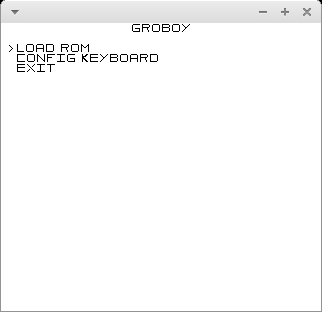
\includegraphics[scale=0.5]{images/screenshot_menu.png}\\
La première option permet à l'utilisateur de choisir un jeu, et donc de naviguer parmis ses dossiers.\\
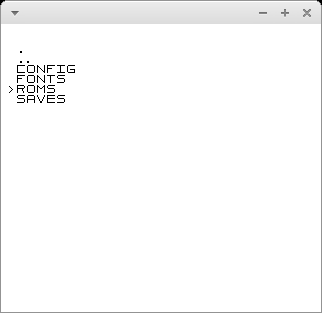
\includegraphics[scale=0.5]{images/screenshot_navigate.png}\\
La seconde option permet à l'utilisateur de configurer les touches.\\
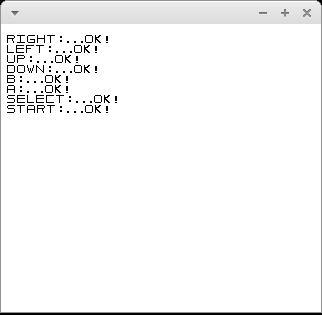
\includegraphics[scale=0.5]{images/screenshot_config.png}\\
La dernière option ne sert juste qu'à quitter l'interface. Enfin une fois le jeu choisi le menu change et propose toujours les différentes options en plus de pouvoir lancer le jeu.\\
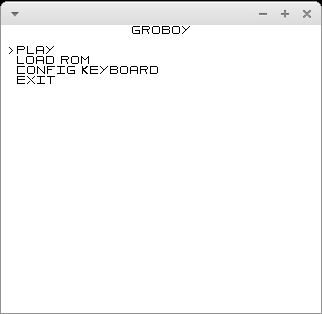
\includegraphics[scale=0.5]{images/screenshot_menu2.png}\\
Nous ne détaillerons pas plus comment nous avons réalisé cette partie car elle n'intervient pas vraiment dans la réalisation d'un émulateur.
\chapter*{Conclusion}
\section*{Bilan}
\section*{Fonctionnalités pouvant être rajoutées}
\section*{Emulation aujourd'hui}
%bibliographie
\bibliographystyle{plain}
\bibliography{rapport}
%annexes
\appendix
\chapter{Comptes rendus de réunion}
\chapter{Générer un son en temps réel et sans fichier avec la SDL}
\chapter{Méthodes de débuggage et roms de test}

\end{document}
